\documentclass{article}
    % General document formatting
    \usepackage[margin=0.6in]{geometry}
    \usepackage[parfill]{parskip}
    \usepackage[utf8]{inputenc}
    
    % Related to math
    \usepackage{amsmath,amssymb,amsfonts,amsthm}
\usepackage{graphicx}
%\usepackage{subfig}
%\usepackage{subfigure}
\usepackage{caption}
\usepackage{subcaption}
\usepackage{listings}
\usepackage[percent]{overpic}
\usepackage{xcolor}

\usepackage{titling}
%\usepackage{lipsum}

\usepackage{titlesec}

\titleformat*{\section}{\large\bfseries}
\titleformat*{\subsection}{\large\bfseries}
%\titleformat*{\subsubsection}{\large\bfseries}
%\titleformat*{\paragraph}{\large\bfseries}
%\titleformat*{\subparagraph}{\large\bfseries}
\titlespacing\section{0pt}{10pt plus 4pt minus 2pt}{0pt plus 2pt minus 2pt}
\titlespacing\subsection{0pt}{12pt plus 4pt minus 2pt}{0pt plus 2pt minus 2pt}
\titlespacing\subsubsection{0pt}{12pt plus 4pt minus 2pt}{0pt plus 2pt minus 2pt}

\pretitle{\begin{center}\large\bfseries}
\posttitle{\par\end{center}\vskip 0.01em}
\preauthor{\begin{center}\Large\ttfamily}
\postauthor{\end{center}}
\predate{\par\normalsize\centering}
\postdate{\par}

%\date{\today}

\begin{document}


%\maketitle

\begin{center}
\textbf{\Large{\centering{FG Assignment 1: Statistical analysis of RNA sequencing data}}}\\
~\\
\textit{USN: 303039534}
\end{center}


\section{Comparison of RNA-seq Data}

The R function simulate.data has been implemented as requested to generate reads from a Poisson distribution (equation 1) whose rate parameter is drawn from a gamma distribution (equation 2).

\begin{equation}
y_{ijk} \sim \text{Pois}(\lambda_{ij})
\end{equation}
\begin{equation}
\lambda_{ij} \sim \text{Gamma}(\alpha_i, \beta_i)
\end{equation}

We can draw $\beta_i$ from a prior gamma distribution with parameters 0.5 and 0.1 (equation 3) or sample from a posterior distribution inferred from a set of reads, with conditional posterior distributions for $\lambda$ and $\beta$ given by equations 5 and 6. For the entirety of this report, we set $\alpha_1 = \alpha_2=100$.
\begin{equation}
\beta_i \sim \text{Gamma}(0.5, 0.1)
\end{equation}
\begin{equation}\tag{5}
P(\lambda_{ij} | \lambda_{-ij},\beta,y) \propto \text{Gamma}(\alpha_i + \sum_k{y_{ijk}}, \beta_i + K)
\end{equation}
\begin{equation}\tag{6}
P(\beta_i | \lambda,\beta_{-i},y) \propto \text{Gamma}(a+\alpha_i J, b+\sum_j{y_{ij}})
\end{equation}
Using simulate.data, a vector of reads for 200 experiments across 10 cell lines in 10 replicates for each lab (J=K=10) is generated and the reads plotted in figure \ref{fig:counts} against experiment number (vector index). For this simulation, we set $\beta_1 = 2$ and $\beta_2 = 3$.

\begin{figure}[h]
	\centering
	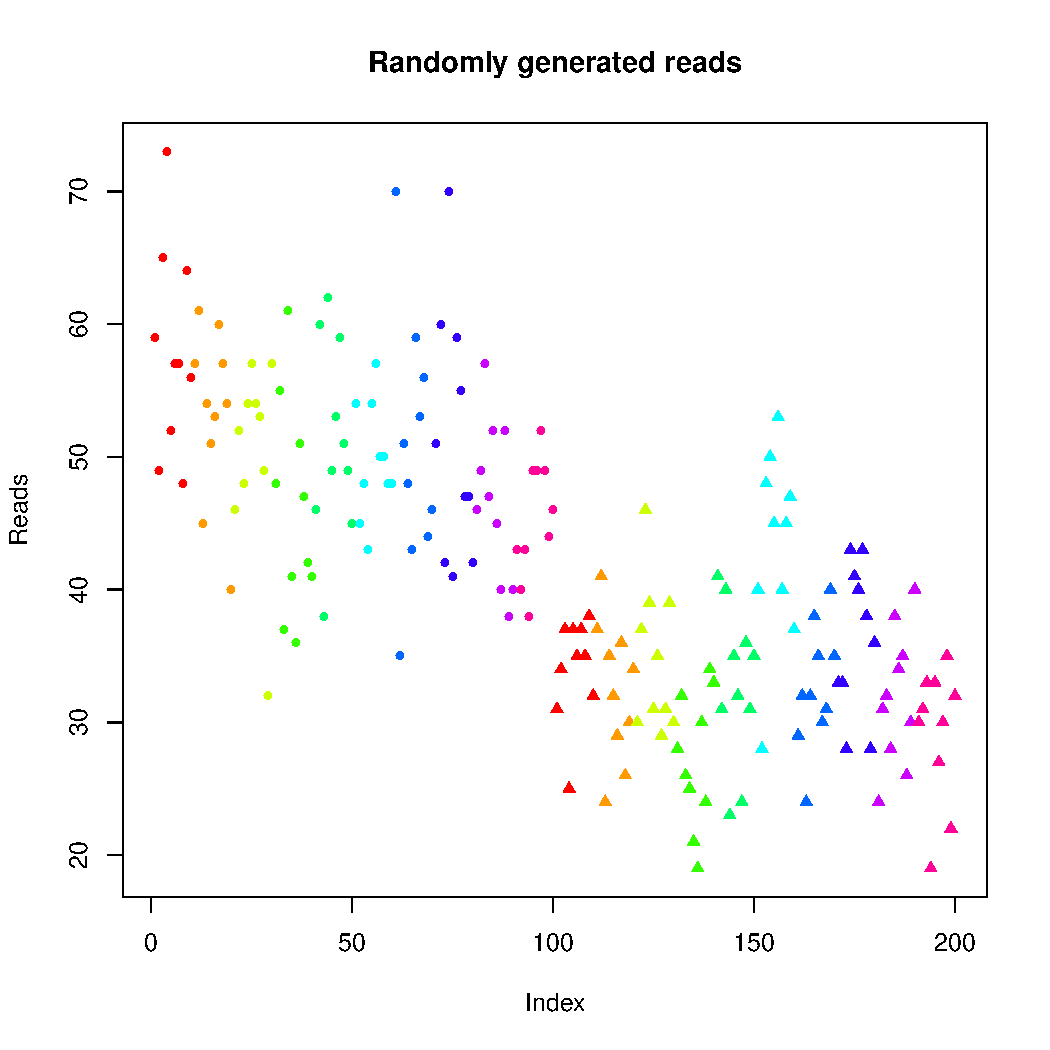
\includegraphics[width = 0.5\linewidth, trim={0 0 0 0}, clip=true]{figs/counts_plot.pdf}
	\caption{Randomly generated counts grouped by cell line by lab. Lab 1 spans reads 1 to 100 (circles), lab 2 reads 101 to 200 (triangles). Each cell line spans 10 experiments.}
	\label{fig:counts}	
\end{figure}

We see that there is variability within each cell line as the reads are drawn randomly from Poisson distribution (1), but the read counts within a cell line tend to be more similar than counts between cell lines due to differences in $\lambda$. We also observe higher reads on average for lab 1 than lab 2 due to the smaller shape parameter. However, despite these trends, there is overlap between most of the read distributions between experiments, emphasizing the need for multiple replicates to infer systematic biases both in the present simulation and real biological experiments.

\newpage

Drawing 100 $\beta$ from (3), we generate a set of 100 $\lambda$ and plot the corresponding Poisson distributions in figure \ref{fig:pois}.

\begin{figure}[h]
	\centering
	\begin{overpic}[width=0.65\textwidth]{figs/many_plots.pdf}
		\put(0,-0.2){\color{blue}\rule{0.065\textwidth}{1pt}}
		%\put(0,10){\color{black}\rule{1pt}{30pt}}
		\put(-0.5,-2.5){\color{blue}\small0}
		\put(6.5,-2.5){\color{blue}\small800}
	\end{overpic}
	\caption{100 Poisson distributions generated by drawing $\lambda$ from (2) setting $\alpha=100$ and drawing $\beta$ from (3). All distributions are normalized and plotted over the range $x=[0:800]$.}
	\label{fig:pois}
\end{figure}

We note that there is a lot of variability between the Possion distributions in figure \ref{fig:pois}. This is a prerequisite for being able to model the orders of magnitude differences in expression levels observed in real biological systems.


The R function gibbs.sampler() has been implemented as specified. This allows us to draw $\beta$ values from (6) given a list of reads and initial guesses of $\beta_i$. We simulate a set of reads with $\beta_1 = 0.12$, $\beta_2 = 0.10$ and $J = K = 10$ and run a Monte Carlo simulation with 5000 iterations using gibbs.sampler with initial parameters $\beta_1 = 0.15$, $\beta_2 = 0.12$ and fixed $\alpha_i= 100$ to infer $\beta_i$. Higher initial $\beta$ values give similar results with up to $\beta_1 = \beta_2 = 10^{100}$ having been tested. The present values have been chosen for convenience of plotting, and the MCMC traces of these simulations are given in figure \ref{fig:MCMC}.

\begin{figure}[h]
	\centering
	\begin{subfigure}[t]{0.47\linewidth}
		\centering
		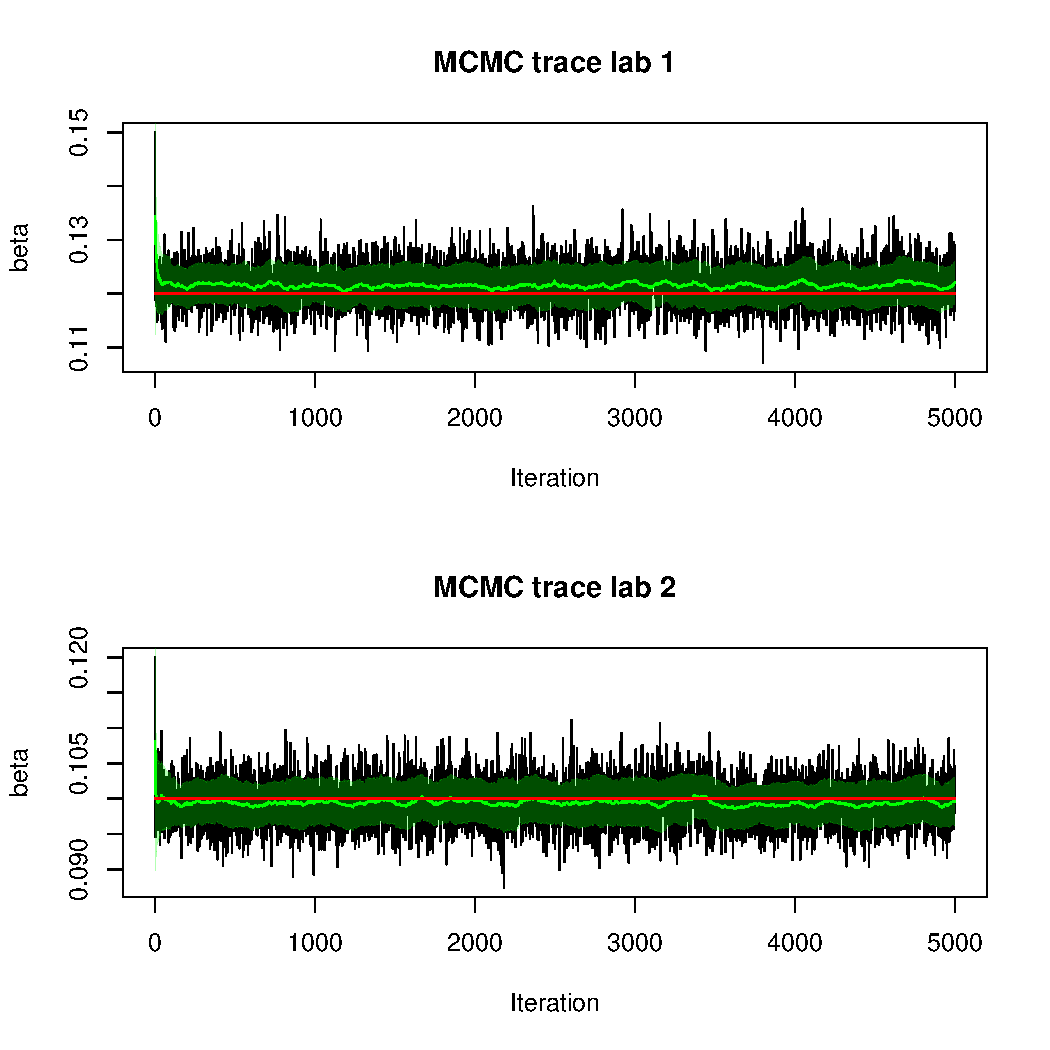
\includegraphics[width=1.0 \linewidth,trim={0 20 10 20}, clip=true]{figs/MCMC_traces.pdf}
		\caption{MCMC traces (black) of $\beta_1$(top) and $\beta_2$ (bottom) with model parameters described in the text. Solid green lines: rolling averages over 100 iterations. Green shaded areas: plus/minus one standard deviation. Solid red lines: true values of $\beta_1 = 0.12$ and $\beta_2 = 0.10$.}
		\label{fig:MCMC}
	\end{subfigure}
	\hfill
	\begin{subfigure}[t]{0.47\linewidth}
		\centering
		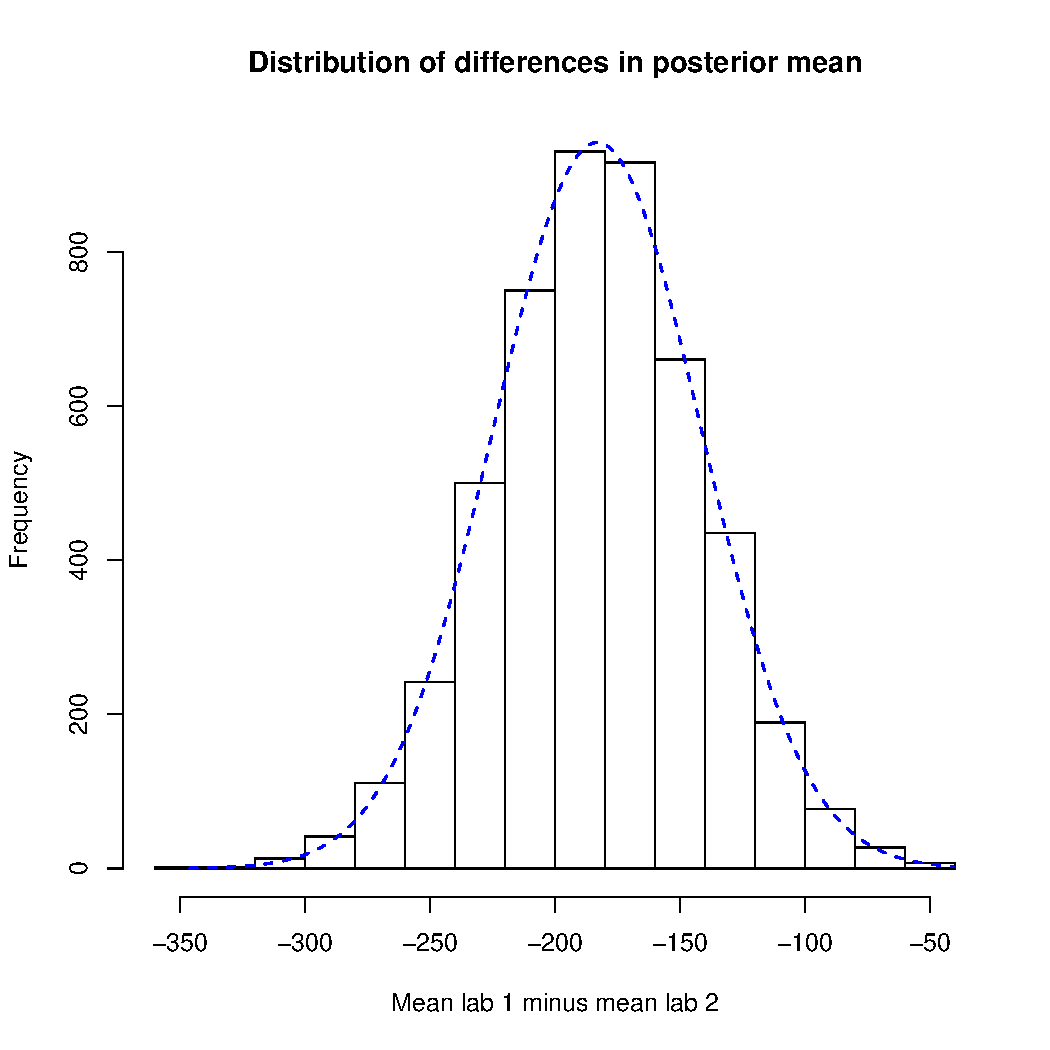
\includegraphics[width=1.0 \linewidth,trim={0 20 10 20}, clip=true]{figs/MCMC_hist_diff.pdf}
		\caption{Histogram of $\dfrac{\alpha_1}{\beta_1} - \dfrac{\alpha_2}{\beta_2}$ at each iteration of the MCMC trace after the burn-in period.  Superimposed on the histogram is a normal distribution fitted to the data.}
		\label{fig:means}
	\end{subfigure}
\end{figure}

%\begin{figure}[h]
%	\centering
%	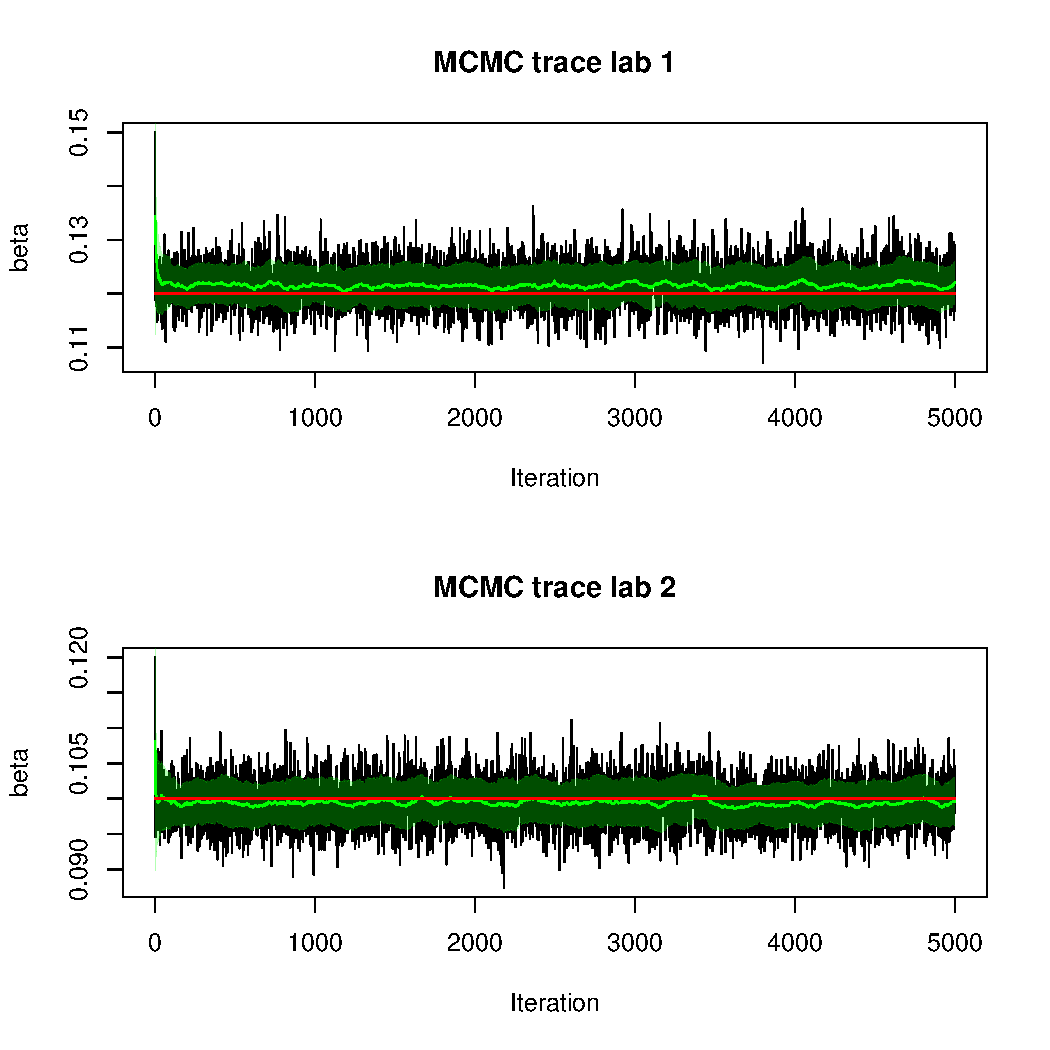
\includegraphics[width = 0.5\linewidth, trim={0 0 0 0}, clip=true]{figs/MCMC_traces.pdf}
%	\caption{MCMC traces (black) of $\beta_1$(top) and $\beta_2$ (bottom) with model parameters described in the text. Superimposed on these traces are rolling averages over iterations (green solid line) plus and minus one standard deviation (green shaded area). Aditionally, the true values of $\beta_1 = 0.12$ and $\beta_2 = 0.10$ are indicated by solid red lines.}
%	\label{fig:MCMC}	
%\end{figure}

From these traces, we see that the model rapidly converges to near the true values of $\beta_1$ and $\beta_2$. The reason for the rapid convergence is that the shape parameter of the Gamma distribution in equation 5 is independent of $\beta_i$, and the rate parameter $\beta_i+K$ is only weakly perturbed by $\beta_i$ since $\beta_i << K$. $\lambda_{ij}$ thus converge in the first iteration, and given these converged rate parameters,  $\beta_i$ also converge.

To asses whether there is evidence to conclude that lab 2 generates more reads than lab 1, we consider at each iteration after a burn-in period of 100 iterations the difference in posterior means of the inferred gamma distributions (equation 2) from which we draw read rate parameters for the two labs. This difference is given by $\dfrac{\alpha_1}{\beta_1} - \dfrac{\alpha_2}{\beta_2}$ (figure \ref{fig:means}).

%\begin{figure}[h]
%	\centering
%	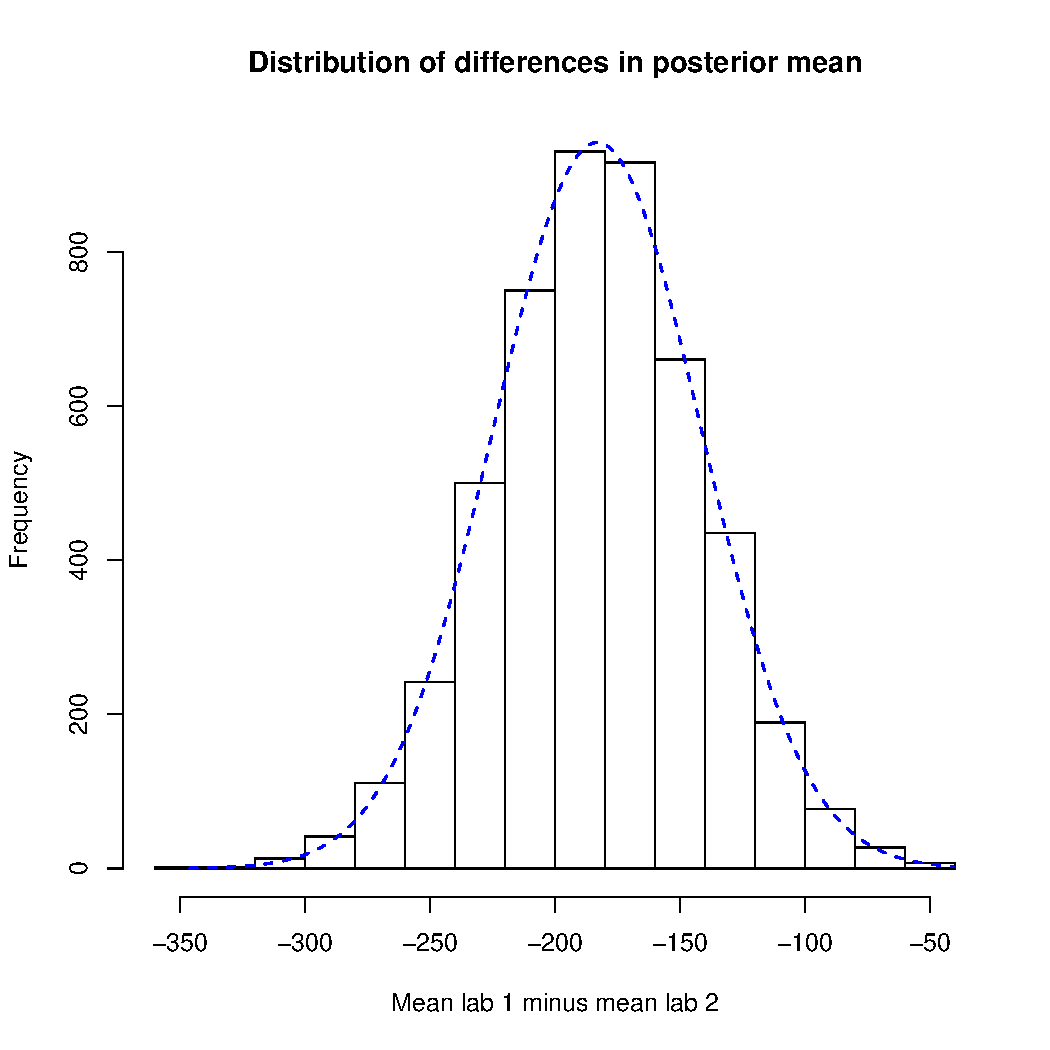
\includegraphics[width = 0.5\linewidth, trim={0 0 0 0}, clip=true]{figs/MCMC_hist_diff.pdf}
%	\caption{Histogram of differences in means between gamma distributions for labs 1 and 2 at each iteration of the MCMC trace after the burnout period.}
%	\label{fig:means}	
%\end{figure}
%
%	One Sample t-test
%
%data:  a1/res[[2]][1, -(1:100)] - a2/res[[2]][2, -(1:100)]
%t = -294.24, df = 4899, p-value < 2.2e-16
%alternative hypothesis: true mean is not equal to 0
%95 percent confidence interval:
% -172.5222 -170.2385
%sample estimates:
%mean of x 
%-171.3804 
%
%
%J = 10 K = 10 p_same = 0 conf -172.5222 -170.2385 
%
%	Shapiro-Wilk normality test
%
%data:  meandiff
%W = 0.99945, p-value = 0.1574
\newpage
The difference in posterior means appears to be normally distributed which we confirm by performing a Shapiro-Wilks test on the data, giving W=0.9997 and p = 0.78 with similarly high W and p values having been generated every time the script has been run. Since the differences are normally distributed, we can run a one-sample t-test to estimate the probability that the real difference in means is less than zero. This gives $p < 2.2\text{E-16}$ (the lowest value that can be reported in R), and we thus conclude that the difference in means of the Gamma distributions is less than zero and hence that lab 1 generates systematically fewer reads than lab 2.

Finally, we consider the effect of increasing J and K on the accuracy and confidence of our predicted beta values in a single trial (figure \ref{fig:distributions}) and over 1000 trials (figure \ref{fig:distributions_screen}).

\begin{figure}[h]
	\centering
	\begin{subfigure}[t]{0.55\linewidth}
		\centering
		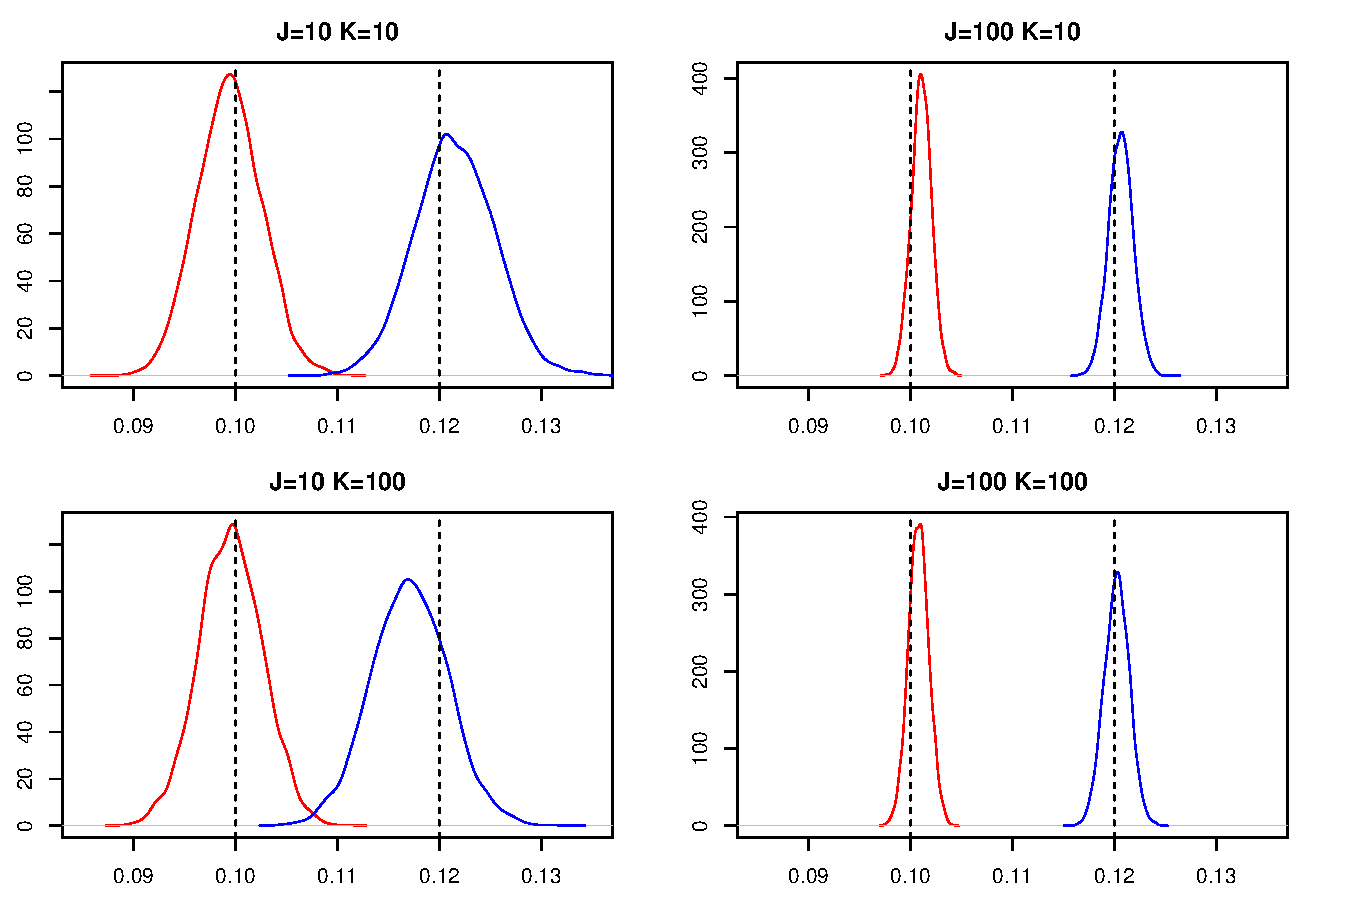
\includegraphics[width = \linewidth, trim={0 0 0 0}, clip=true]{figs/screen_distributions.pdf}
		\caption{Distributions of beta values for different combinations of J and K values. Distributions for lab 1 are given in blue, lab 2 in red. Vertical dashed lines indicate true values.}
		\label{fig:distributions}
	\end{subfigure}	
	\hfill
	\begin{subfigure}[t]{0.366\linewidth}
		\centering
		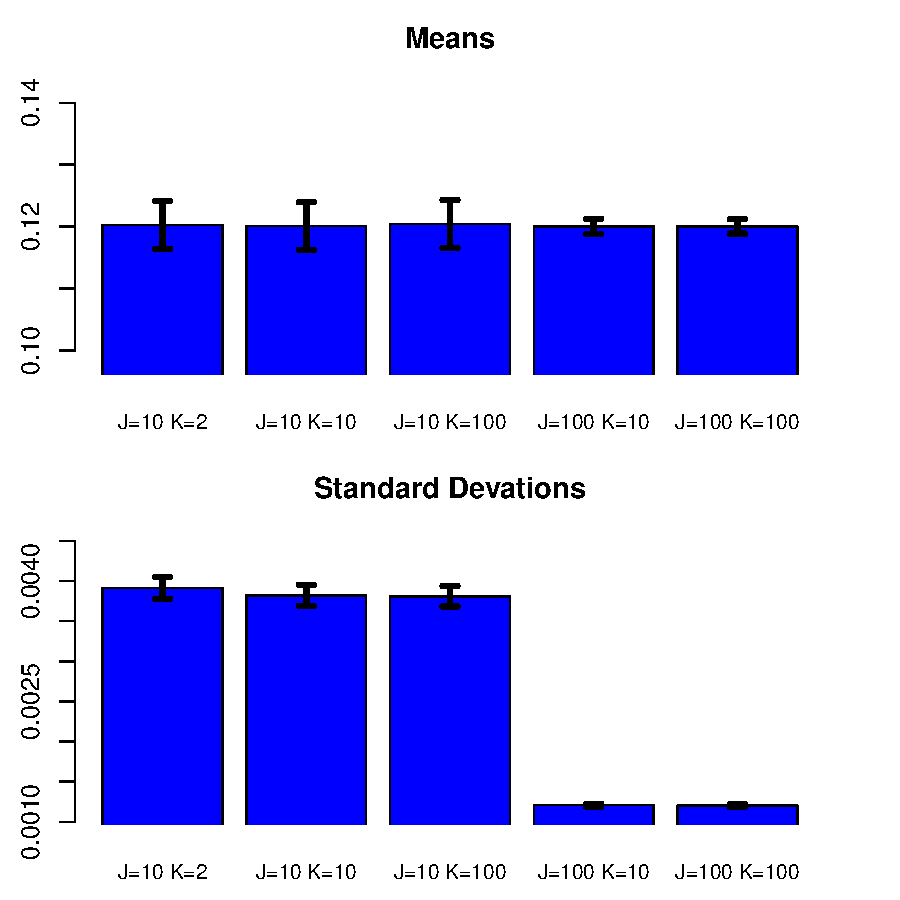
\includegraphics[width = \linewidth, trim={0 0 0 0}, clip=true]{figs/repeat_screen.pdf}
		\caption{Means (top) and standard deviations (bottom) of $\beta_1$ distributions in (a) for 1000 simulations. Error bars are 1 standard deviation.}
		\label{fig:distributions_screen}
	\end{subfigure}	
\end{figure}


In general, we observe that increasing J leads to less fluctuations (lower variance) and thus more confidence in the $\beta$ values; i.e. a narrower posterior distribution. This is because we draw more $\beta$ values from the true distribution which helps pinpoint the real values. We see this in equation 6 where increasing J leads to a proportional increase in both the shape and rate parameters of the conditional posterior distribution from which we draw $\beta$ since $\alpha_i >> a$ and $\sum_j{\lambda_{ij}} >> b$. The mean is thus unaffected by this scaling while the variance decreases since scaling $J$ to $c J$ gives:\\
%\begin{centering}
$\text{Var}(\beta | cJ) =\dfrac{\alpha_{cJ}}{{(\beta_{cJ})}^2} = \dfrac{c\, \alpha_J}{{(c\, \beta_J )}^2} = \dfrac{1}{c} \dfrac{\alpha_J}{{\beta_J}^2} = \dfrac{1}{c}\text{Var}(\beta | J)$ \\
%\end{centering}
Hence the variance of the conditional posterior distribution (6) is inversely proportional to J within the parameter space investigated. This implies that the standard deviation decreases as $\sqrt{c}$ which is confirmed in figure \ref{fig:distributions_screen} where the mean fold change going from J = 100 to J = 10 is is just 0.1\% from the expected value of $\sqrt{10}$.

From equation 5, we see that increasing K decreases the variance of $\lambda$ since both parameters of the conditional posterior distribution for lambda (equation 5) are approximately proportional to K:\\
%\begin{centering}
$E(\sum_k{\lambda_{ijk}}) = \sum_k{E(\lambda_{ijk})} = K E(\lambda_{ij}) >> \alpha ~~~$     and      $~~~K >> \beta$\\
%\end{centering}
However, the only term that goes into equation 6 is the sum of $\lambda_{ij}$ over j, the expectation value of which is independent of the variance of $\lambda$. For large values of K where this is true, we thus do not expect K to affect the variance of $\beta_i$.

Indeed, looking at figure \ref{fig:distributions_screen}, increasing K appears to have only little effect on the mean or variance of $\beta$. There is no observable difference between K=10 and K=100 for J=10 or J=100, and even decreasing K to 2 yields only a small increase in the mean and variance of $\beta$. In the K=2 case, $\alpha_1 \approx 0.06 E(\sum_k{\lambda_{1jk}}) $ so the above analysis no longer holds as the scaling of the shape parameter with K in (5) is now sub-linear. This leads to a reduced mean of the corresponding gamma distribution, a decrease in $E(\lambda)$ and corresponding decrease in the rate parameter $\alpha_{(6)} = b + \sum_j{\lambda_j}$ of equation (6). This results in an increased mean and variance of the conditional posterior distribution of $\beta$ with decreasing K as observed in figure \ref{fig:distributions_screen}.

Note that in figure \ref{fig:distributions_screen}, the error bar on the estimated means (top) tells us how consistently we estimate beta, whereas the mean of the standard deviations (bottom) tells us how confident we think we are of $\beta$ in a given trial. It is possible for the single-trial distribution of $\beta$ to be narrow yet inaccurate, which would lead to a high standard deviation of the means yet a low mean standard deviation. However, the two parameters are consistent in the present case.

\section{Adequacy of Experimental Design and Modeling}

In the present experimental setup, the two labs are each assigned J random cell lines without replacement. In order to use the resulting read information to infer lab-specific biases, we must thus assume that the two sets of cell lines $\{J_{1k}\}$ \& $\{J_{2k}\}$ have on average the same inherent expression level since any bias detected may otherwise be due to differences between the sets of cell lines sequenced rather than a systematic difference between the labs. A more appropriate experiment might be to select J cell lines at random and then give both labs a culture of the \textit{same} set of cell lines for sequencing in K replicates. We can then do a pairwise comparison of the inferred expression levels for each of the J cell lines across the K replicates and assess whether there is a systematic difference in read generation between the two labs.

We draw $\lambda$ values for each cell line from a relatively narrow unimodal gamma distribution and use these to draw reads from the corresponding Poisson distributions. This may not reflect biological reality where many genes may follow broader or even multi-modal distributions across cell lines. This reflects the fact that there is a high degree of variation in gene expression for many non-essential genes, and that this is in some cases near-binary e.g. for regulatory genes. For example, Fred Davis et al. recently modeled neurotransmitter and receptor expression in a bimodal framework to infer binary functionality in fly neurons, and their experimental expression levels do not appear to follow a gamma distribution (Davis et al. bioRxiv (2018) https://doi.org/10.1101/385476 ). By using a unimodal gamma distribution, we may thus underestimate biological variability. This will also lead to an underestimate of the effect of the aforementioned variation between cell lines, and this potential deficiency of the model may thus mask experimental inadequacies.

In order to extend the method above to multiple genes (i.e. using information from multiple genes to determine whether there is a consistent bias between labs), I would conduct two analyses:
\begin{enumerate}
\item
I would sample the mean difference between posterior means,  $E(\alpha_1 / \beta_1 - \alpha_2 / \beta_2 )$, across genes and assess whether the resulting distribution is significantly different from zero after discarding genes with very low expression across labs. I would do this on differences normalized e.g. by average read count. The particular statistical test of choice would depend on what the distribution of normalized mean differences looks like. This analysis would indicate whether there is a systematic difference in inferred expression levels across genes.
\item
Using Bonferroni-corrected p-values from one-sample t-tests on the distributions of differences in posterior means (figure \ref{fig:means}) for each gene, I would count the number of genes for which lab 1 generates more reads than lab 2 and vice versa. The fraction of genes for which there is a significant difference is a measure of general variability between the labs, whereas the relative number of enriched genes for lab 1 compared to lab 2 and vice versa is an indicator of systematic bias. In both of these analyses, I have assumed that expression levels of different genes are independent, which is of course not entirely true but simplifies our analyses greatly.

\end{enumerate}







%\begin{figure}[h]
%	\centering
%	\begin{subfigure}[t]{0.32\linewidth}
%		\centering
%		\includegraphics[width=1.0 \linewidth,trim={0 10 50 60}, clip=true]{../figs/hist_kmer57_cut0.pdf}
%		\caption{Raw histogram cov\_cutoff=0 }
%		\label{fig:0raw}
%	\end{subfigure}
%	\begin{subfigure}[t]{0.32\linewidth}
%		\centering
%		\includegraphics[width=1.0 \linewidth,trim={0 10 50 60}, clip=true]{../figs/weighthist_kmer57_cut0.pdf}
%		\caption{Weighted histogram cov\_cutoff=0 }
%		\label{fig:0weight}
%	\end{subfigure}
%	\begin{subfigure}[t]{0.32\linewidth}
%		\centering
%		\includegraphics[width=1.0 \linewidth,trim={0 10 50 60}, clip=true]{../figs/weighthist_kmer57_cut7.pdf}
%		\caption{Weighted histogram cov\_cutoff=7 }
%		\label{fig:7weight}
%	\end{subfigure}
%\label{fig:hist_noparams}
%
%\end{figure}
 
\end{document}